\documentclass[border=0.2pt]{standalone}
\usepackage{tikz,times}
\usetikzlibrary{patterns}
\begin{document}

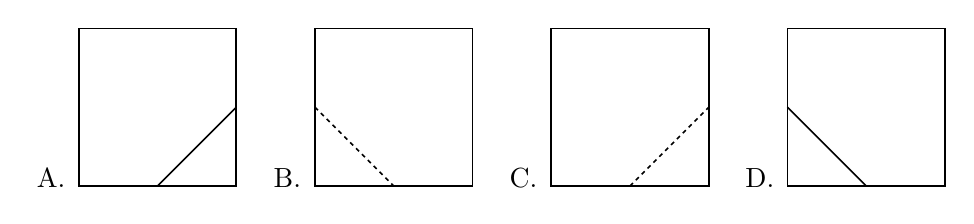
\begin{tikzpicture}[line width=0.6pt]

\draw(0,0)node[left=10pt,above=-4pt]{A.} rectangle (2,2);
\draw(1,0)--(2,1);

\draw(3,0)node[left=10pt,above=-4pt]{B.} rectangle (5,2);
\draw[dash pattern=on 1.5pt off 1.5pt](3,1)--(4,0);

\draw(6,0)node[left=10pt,above=-4pt]{C.} rectangle (8,2);
\draw[dash pattern=on 1.5pt off 1.5pt](7,0)--(8,1);

\draw(9,0)node[left=10pt,above=-4pt]{D.} rectangle (11,2);
\draw(9,1)--(10,0);

\end{tikzpicture}


\end{document} 